\section{Source Selection}
The system is designed to take in three parameters, a list of all source points in the space, the dimensions of the space the points lie in and the intensity threshold. Each element of the list of sources has 3 parameters: x, y and z. The x and y parameters define the spatial coordinates of the source while the z parameter is seen as the intensity of the source, the list of $n$ sources are passed into the function as an $n \times 3$ numpy array of doubles. The spatial dimension parameter takes in a tuple of two values, the width and height of the space the sources are in. The intensity threshold is a single double value which defines the minimum intensity a source needs to be a voronoi cell centre.
\\
\\
The sources are read in and are used to generate the voronoi centres as a points. Each point inherits the x, y and z values of the source and the rest are kept as default values. Once the list of points is created, it is sorted by the x then the y values of the sources. Once the centre points are generated, generation the voronoi diagram can begin.
\\
\\
For the sake of testing the system the coordinates are randomly generated on a $600 \times 600$ plane with the intensity randomly generated as the absoulute value of a random normal distribution, centred at zero with a standard deviation of $3000$. Using this, 10000 sources are randomly generated. From these sources, we generate centres to be used by the Voronoi, centres are sources with an intensity greater than one standard deviation of the original mean, since the absoulute value of the source intensity is used, this is all points with an intensity greater than 3000, this accounts for approximately $32\%$ of the sources.
\begin{figure}[H]
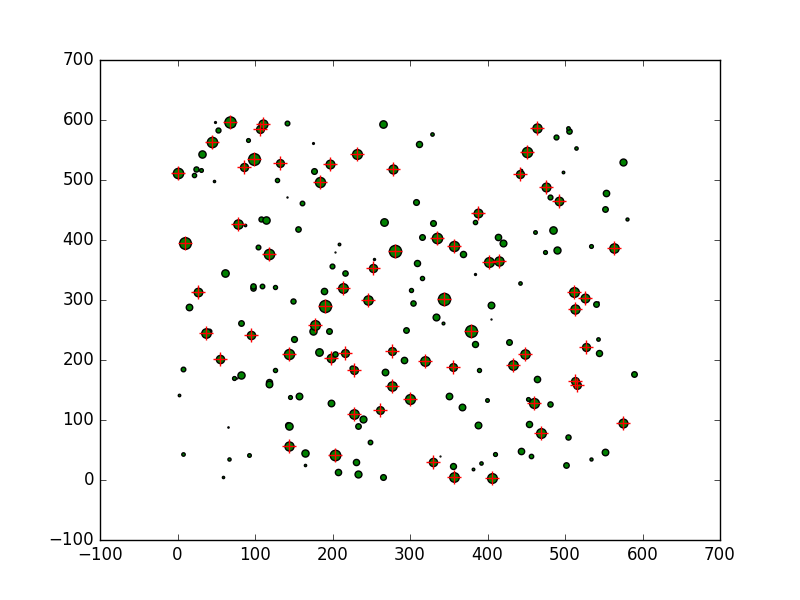
\includegraphics[width=\textwidth]{Images/sources.png}
\caption{Sources and selected centres.}
\label{fig:source}
\end{figure}
Figure \ref{fig:source} shows sources in green with their intensities representing the radius of the on the plane, to simplify, only $200$ points are generated. The crosses in red represent the centres that will be used to generate the Voronoi tessellation.